\msection{Offensive Diversification: Malware evasion}

The primary malicious use of WebAssembly in browsers is cryptojacking \cite{musch2019new}. 
This is due to the essence of cryptojacking, the faster the mining, the better. 
Although the research of Lehmann and colleagues \cite{Hilbig2021AnES} suggests a decline in browser-based cryptominers, mainly due to the shutdown of Coinhive, a 2022 report by Kaspersky indicates that the use of cryptominers is on the rise \cite{kasperksy}. 
This underscores the ongoing need for effective automatic detection of cryptojacking malware.

Both antivirus software and browsers have implemented measures to detect cryptojacking. For instance, Firefox employs deny lists to detect cryptomining activities \cite{firefoxcrypto}. 
The academic community has also contributed to the body of work on detecting or preventing WebAssembly-based cryptojacking, as outlined in \autoref{background:wasm:analysis}. 
However, it's worth noting that malicious actors can employ evasion techniques to circumvent these detection mechanisms. 
Bhansali et al. are among the first who have investigated how WebAssembly cryptojacking could potentially evade detection \cite{10.1145/3507657.3528560}, highlighting the critical importance of this use case. 
For an in-depth discussion on this topic, we direct the reader to our contribution \cite{EVASION}.
The use of case illustrated in the subsequent sections uses Offensive Software Diversification for the sake of evading malware detection in \Wasm. 


\msubsection{Threat model}

Let us illustrate the threat model in which a malicious \wasm binary could be involved.
\autoref{fig:threat_model} illustrates a browser attack scenario:
a practical WebAssembly cryptojacking attack consists of three components: a WebAssembly binary, a JavaScript wrapper, and a backend cryptominer pool. 
The WebAssembly binary is responsible for executing the hash calculations, which consume significant computational resources. 
The JavaScript wrapper facilitates the communication between the WebAssembly binary and the cryptominer pool.
Overall, a successful cryptojacking attack on a victim's browser consists in the following sequence of steps. 
First, the victim visits a web page infected with the cryptojacking code. 
The web page establishes a channel to the cryptominer pool, which then assigns a hashing job to the infected browser. 
The WebAssembly cryptominer calculates thousands of hashes inside the browser, in parallel using multiple browser workers. 
Once the malware server receives acceptable hashes, it is rewarded with cryptocurrencies for the mining. 
Then, the server assigns a new job, and the mining process starts over.

\begin{figure}
    \centering
    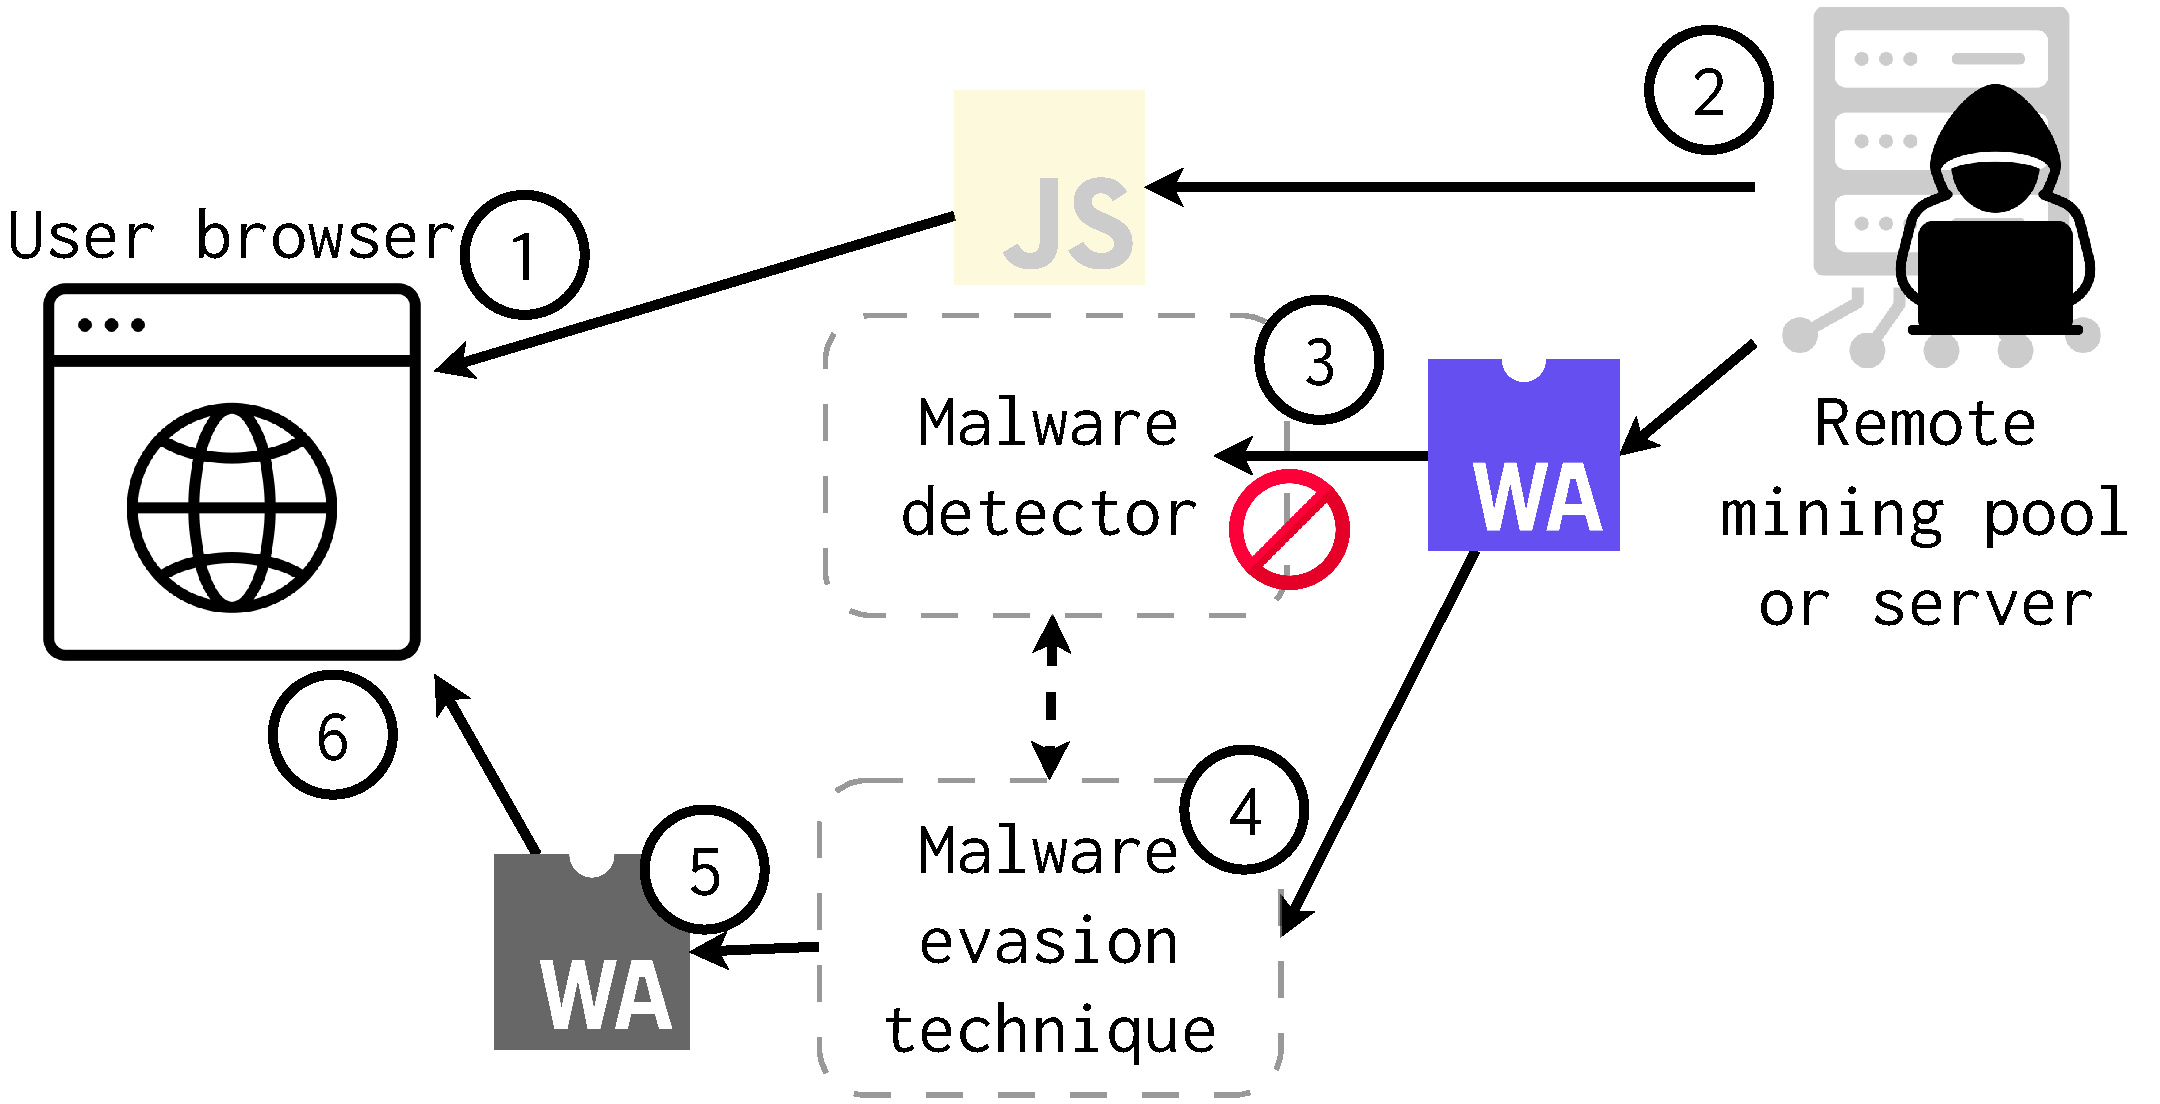
\includegraphics[width=0.8\linewidth]{figures/threat_model.pdf}
    \caption{Taken from \cite{EVASION}}
    \label{fig:threat_model}
\end{figure}

Some detection techniques discussed in \autoref{background:wasm:analysis} can be  deployed in the browser directly to prevent cryptojacking.
The primary objective of our work is to demonstrate the possibility of using code diversification to bypass cryptojacking defenses. 
Concretely, the following workflow can happen to successfully evade placed defenses:

\begin{enumerate}
    
    \item The user visits a webpage that contains a cryptojacking malware, which utilizes network resources to execute, (1) and (2) in \autoref{attack-model}. Cryptojacking malware can be injected through malicious browser extensions, malvertising, compromised websites, or deceptive links \cite{9566204}. 
    \item A malware detector blocks WebAssembly binaries that are identified as malicious (3). The malware detector system can be implemented locally or remotely. For instance, a proxy can intercept and send network resources to an external detector through the detector's API. 
    \item The attacker, based on a malware oracle, crafts a WebAssembly cryptojacking malware variant that evade the detection (4). 
    \item The attacker delivers the modified binary instead of the original one (5), which initiates the cryptojacking process and compromises the browser (6).
\end{enumerate}


The idea is that attackers rapidly diversify their WebAssembly code to stay ahead of the defense system and maintain successful cryptojacking operations. 
Crucially, attackers must ensure that the diversified binaries they use for cryptojacking meet specific performance requirements.
This requirement is why we chose diversification over obfuscation.  
Obfuscation tools can generate program variants that are slower and less performant than the original program \cite{HOSSEINZADEH201872}.  
In contrast, our WebAssembly diversifiers can be tuned to generate variants that span the full performance spectrum, from faster to slower as highlighted.

\todo{Detail the threat model and make a clear statement of the objective of this use case.}

Test and evade the resilience of \Wasm malware detectors mentioned in \autoref{background:wasm:ecosystems}.


\msubsection{Approach}


We evaluate our proposed evasion technique on 33 cryptojacking malware that we curated from the 8643 binaries of the wasmbench dataset \cite{Hilbig2021AnES}, to our knowledge, the most exhaustive collection of real-world WebAssembly binaries.
We experiment with the 33 binaries marked as potentially dangerous by at least one antivirus vendor of VirusTotal.
We empirically demonstrate that evasion is possible for all of these 33 real-world WebAssembly cryptojacking malware while using a WebAssembly-specific detector. 
Remarkably, we find 30 cryptominers for which our technique successfully generates variants that evade VirusTotal.
Our set of malware includes 6 cryptojacking programs that are fully reproducible in a controlled environment. 
With them, we assess that our evasion method does not affect malware correctness and generates fully functional malware variants with minimal overhead.

Our work provides evidence that the malware detection community has opportunities to strengthen the automatic detection of cryptojacking WebAssembly malware. 
The results of this work are actionable, as we provide quantitative evidence on specific malware transformations on which detection methods can focus.

\todo{Mention the uncontrolled and controlled diversification. What are the difference between them. Make a statement about that obfuscation is a face of diversificaation. Specifically, controlled diversification.}

%\lipsum[1]

\todo{We use wasm-mutate}
\todo{How do we use it?}
\todo{Controlled and uncontrolled diversification.}

%\lipsum[1]

%\lipsum[1]

\msubsection{Results}


\begin{tcolorbox}[title=Contribution paper,boxrule=1pt,arc=.2em,boxsep=1.0mm]
    The case discussed in this section is fully detailed in Cabrera-Arteaga \etal "WebAssembly Diversification for Malware Evasion"
    \emph{at Computers \& Security, 2023}
    \url{https://www.sciencedirect.com/science/article/pii/S0167404823002067}. 
\end{tcolorbox}


\emph{Discussion}
In this section we mention some challenges we face during the writing of this work.
We enumerate them in order to enforce the debase and the discussion on the topic.

\emph{Oracle classification moves in time:}
One could expect that the more detectors a binary has, the more iterations are needed to evade them.
However, we have observed that this is not the case for some binaries.
The main reason is that the final labelling of binaries for VirusTotal vendors is not immediate \cite{251586}. 
For example, a VirusTotal vendor could label a binary as benign and change it later to malign after several weeks in a conservative way of acting.
This phenomenon creates a time window in which slightly changed binaries (fewer iterations in our case) could evade the detection of numerous vendors.

\emph{Lack of bigger picture:} A WebAssembly cryptomalware can only exist with its JavaScript complement.
For example, a browser cryptonalware needs to send the calculated hashes to a cryptocurrency service.
This network communication is outside the WebAssembly accesses and needs to be delegated to a JavaScript code.
Besides, other functionalities can be intermixing between JavaScript and WebAssembly and in some cases be completely in one side or the other \cite{romano2022wobfuscator}.
This intermixing between JavaScript and WebAssembly could provide statically different WebAssembly. 
% What we saw
We have observed that, the imports and the memory data of the WebAssembly binaries have a high variability in our original dataset.
The imported functions from JavaScript change from binary to binary.
Their data segments can also differ in content and length.
To completely analyze these cases, the whole JavaScript-WebAssembly program is needed, something only provided in 9/33 cases of our dataset.

\emph{More narrowed fitness function:} We use a simple fitness function, but the MCMC evasion algorithm could have a fitness function as general as wanted.
In our case, we do not use binary metadata, instead we focus on the result from the malware oracle, given that the main goal is to evade this oracle.

\emph{Mitigation: } \todo{TBD, data augmentation, better resilience evaluation ?}


Another interesting thing would be to see if there is difference in the detectors. If some detectors are fooled by some transformations or are more robust, etc.

\todo{Motivate the use case with the following sota}

\wrule{Binary rewriting tools and obfuscators} The landscape for tools that can modify, obfuscate, or enhance \Wasm binaries for various has increased. 
For instance, BREWasm\cite{BREWasm} provides a comprehensive static binary rewriting framework specifically designed for \Wasm. 
Wobfuscator\cite{wobfuscator} takes a different approach, serving as an opportunistic obfuscator for Wasm-JS browser applications. 
Madvex\cite{madvex} focuses on modifying \Wasm binaries to evade malware detection, with its approach being limited to alterations in the code section of a \Wasm binary. 
Additionally, WASMixer\cite{wasmixer} obfuscates WebAssembly binaries, by including memory access encryption, control flow flattening, and the insertion of opaque predicates.


\todo{ The malware evasion paper}
